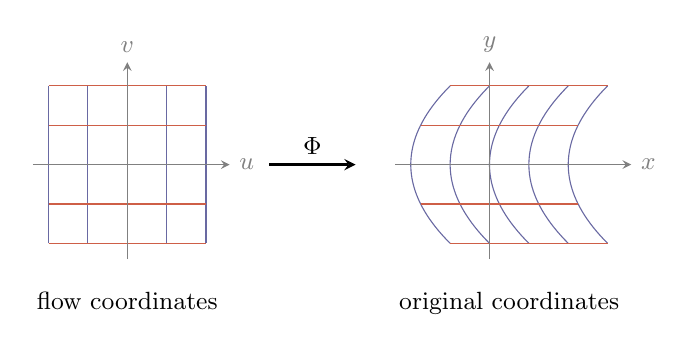
\begin{tikzpicture}[x=1cm,y=1cm,font=\small,>=stealth]
\begin{scope}
\foreach \u in {-1,-.5,0,.5,1} {\draw[MidnightBlue!65] (\u,-1)--(\u,1);}
\foreach \v in {-1,-.5,0,.5,1} {\draw[BrickRed!65] (-1,\v)--(1,\v);}
\draw[gray,->] (-1.2,0)--(1.3,0) node[right] {$u$};
\draw[gray,->] (0,-1.2)--(0,1.3) node[above] {$v$};
\node[below] at (0,-1.5) {flow coordinates};
\end{scope}
\draw[->,thick] (1.8,0)--node[above] {$\Phi$}(2.9,0);
\begin{scope}[shift={(4.6,0)}]
\foreach \u in {-1,-.5,0,.5,1} {
\draw[MidnightBlue!65,domain=-1:1,samples=40] plot ({\u+.5*\x*\x},\x);}
\foreach \v in {-1,-.5,0,.5,1} {
\draw[BrickRed!65] ({-1+.5*\v*\v},\v)--({1+.5*\v*\v},\v);}
\draw[gray,->] (-1.2,0)--(1.8,0) node[right] {$x$};
\draw[gray,->] (0,-1.2)--(0,1.3) node[above] {$y$};
\node[below] at (.25,-1.5) {original coordinates};
\end{scope}
\end{tikzpicture}
